% =====================================================================
%  UROP project report -- Side-burnt document line completion
%  Compile with pdfLaTeX (Overleaf: upload the report/ folder, compile main.tex).
%  Fill in the names below; everything else is generated from the project.
% =====================================================================
\documentclass[12pt,a4paper,oneside]{report}

% ---------- people (edit these) ----------
\newcommand{\ProjectTitle}{Side-Burnt Document Line Completion: Separating What the Image Can Read from What Context Can Only Suggest}
\newcommand{\ShortTitle}{Side-Burnt Document Line Completion}
\newcommand{\StudentA}{Praveen}\newcommand{\RegA}{AP23110010460}
\newcommand{\StudentB}{Pranav}\newcommand{\RegB}{AP23110010457}
\newcommand{\StudentC}{Samad}\newcommand{\RegC}{AP23110010747}
\newcommand{\GuideName}{Dr. Ravi Kant Kumar}
\newcommand{\HodName}{Dr. V M Manikandan}
\newcommand{\SubmitMonth}{December 2026}
\newcommand{\DeclDate}{\today}

% ---------- packages ----------
\usepackage[T1]{fontenc}
\usepackage[utf8]{inputenc}
\usepackage{amsmath}                  % before newpxmath; newpxmath already provides the amssymb symbols
\usepackage{newpxtext,newpxmath}      % Palatino, as in the department template
\usepackage[left=1.25in,right=1in,top=1in,bottom=1in]{geometry}
\usepackage{setspace}
\usepackage{graphicx}
\usepackage{booktabs,tabularx,multirow,array}
\usepackage{caption,subcaption}
\usepackage{xcolor}
\usepackage{tikz}
\usetikzlibrary{arrows.meta,positioning,fit,backgrounds}
\usepackage{titlesec}
\usepackage{enumitem}
\usepackage{float}
\usepackage[hidelinks]{hyperref}
\usepackage[nottoc]{tocbibind}

\graphicspath{{figures/}}
\setstretch{1.4}
\setlength{\parindent}{2em}
\captionsetup{font=small,labelsep=colon}
\definecolor{cblue}{HTML}{2A78D6}
\definecolor{corange}{HTML}{EB6834}
\definecolor{caqua}{HTML}{1BAF7A}
\definecolor{cgray}{HTML}{8A8984}

% Chapter headings centred: "Chapter n" over the upper-case title, as in the template
\titleformat{\chapter}[display]{\centering\bfseries}{\Large\chaptertitlename\ \thechapter}{4pt}{\LARGE\MakeUppercase}
\titlespacing*{\chapter}{0pt}{30pt}{24pt}
\titleformat{\section}{\large\bfseries}{\thesection}{1em}{\MakeUppercase}
\titleformat{\subsection}{\normalsize\bfseries}{\thesubsection}{1em}{}

\newcommand{\logo}[1]{\IfFileExists{figures/srm_logo.png}{\includegraphics[width=#1]{srm_logo.png}}{\fbox{\parbox[c][#1][c]{#1}{\centering\footnotesize SRM logo\\(figures/srm\_logo.png)}}}}
\newcommand{\READ}{\texorpdfstring{\textsc{read}}{READ}}
\newcommand{\INF}{\texorpdfstring{\textsc{inferred}}{INFERRED}}

\begin{document}

% =====================================================================
%  Title page
% =====================================================================
\begin{titlepage}
\centering\setstretch{1.25}
{\large\bfseries \MakeUppercase{\ShortTitle}\par}
\vspace{1.5em}
Project Report Submitted to the\\
SRM University-AP, Andhra Pradesh\\
for the partial fulfillment of the requirements to award the degree of\par
\vspace{1.2em}
{\bfseries Bachelor of Technology\\ in\\ Computer Science \& Engineering\\ School of Engineering \& Sciences\par}
\vspace{1.2em}
submitted by\par\vspace{0.6em}
{\bfseries \StudentA\ (\RegA)\\[0.3em] \StudentB\ (\RegB)\\[0.3em] \StudentC\ (\RegC)\par}
\vspace{1.2em}
Under the Guidance of\par\vspace{0.4em}
{\bfseries \GuideName\par}
\vspace{1.5em}
\logo{3.2cm}\par
\vspace{1.5em}
{\large\bfseries Department of Computer Science \& Engineering\par}
SRM University-AP\\ Neerukonda, Mangalgiri, Guntur\\ Amaravati, Andhra Pradesh - 522 240\\[0.3em]
{\large \SubmitMonth\par}
\end{titlepage}

% =====================================================================
%  Declaration / Certificate
% =====================================================================
\pagenumbering{roman}\setcounter{page}{2}
\chapter*{Declaration}
I undersigned hereby declare that the project report \textbf{\ShortTitle} submitted for
partial fulfillment of the requirements for the award of degree of Bachelor of Technology in
the Computer Science \& Engineering, SRM University-AP, is a bonafide work done by me under
supervision of \GuideName. This submission represents my ideas in my own words and where ideas
or words of others have been included, I have adequately and accurately cited and referenced the
original sources. I also declare that I have adhered to ethics of academic honesty and integrity
and have not misrepresented or fabricated any data or idea or fact or source in my submission.
I understand that any violation of the above will be a cause for disciplinary action by the
institute and/or the University and can also evoke penal action from the sources which have thus
not been properly cited or from whom proper permission has not been obtained. This report has not
been previously formed the basis for the award of any degree of any other University.

\vspace{3em}\noindent
\begin{tabular}{@{}llll@{}}
Place & : Amaravati & Date & : \DeclDate\\[0.6em]
Name of student & : \StudentA & Signature & : \makebox[10em]{\dotfill}\\[0.6em]
Name of student & : \StudentB & Signature & : \makebox[10em]{\dotfill}\\[0.6em]
Name of student & : \StudentC & Signature & : \makebox[10em]{\dotfill}\\
\end{tabular}

\clearpage
\thispagestyle{plain}
\begin{center}\setstretch{1.25}
{\large\bfseries DEPARTMENT OF COMPUTER SCIENCE \&\\ ENGINEERING\\ SRM University-AP\\
Neerukonda, Mangalgiri, Guntur\\ Amaravati, Andhra Pradesh - 522 240\par}
\vspace{1.5em}\logo{2.4cm}\par\vspace{1.5em}
{\large\bfseries CERTIFICATE\par}
\end{center}
This is to certify that the report entitled \textbf{\ShortTitle} submitted by
\textbf{\StudentA, \StudentB, \StudentC} to the SRM University-AP in partial fulfillment of
the requirements for the award of the Degree of Bachelor of Technology in the Department of
Computer Science \& Engineering is a bonafide record of the project work carried out under
my/our guidance and supervision. This report in any form has not been submitted to any other
University or Institute for any purpose.

\vspace{5em}\noindent
\begin{tabular}{@{}l@{\hspace{5em}}l@{}}
Project Guide & Head of Department\\[0.5em]
Name\ \ : \GuideName & Name\ \ : \HodName\\[0.5em]
Signature: \dots\dots\dots\dots\dots & Signature: \dots\dots\dots\dots\dots\\
\end{tabular}

% =====================================================================
%  Front matter
% =====================================================================
\clearpage
\chapter*{Acknowledgment}
\addcontentsline{toc}{chapter}{ACKNOWLEDGMENT}
We wish to record our indebtedness and thankfulness to all who helped us prepare this project
report titled \textbf{\ShortTitle} and present it satisfactorily.

We are especially thankful to our guide and supervisor \GuideName\ in the Department of Computer
Science \& Engineering for valuable suggestions and critical inputs in the preparation of this
report. We are also thankful to \HodName, Head of the Department of Computer Science \&
Engineering, for encouragement.

The texts used in this work come from Project Gutenberg, whose volunteers have made thousands of
public-domain books freely available. Our friends in class have always been helpful, and we are
grateful to them for patiently listening to our presentations on this project.

\vspace{3em}
\begin{flushright}\setstretch{1.2}
\StudentA, \StudentB, \StudentC\\
(Reg. No. \RegA, \RegB, \RegC)\\
B.\,Tech.\\ Department of Computer Science \& Engineering\\ SRM University-AP
\end{flushright}

\chapter*{Abstract}
\addcontentsline{toc}{chapter}{ABSTRACT}
When the edge of a printed page burns, the ends of its lines are lost. Near the burn front
the ink is not gone at once: a band of darkened paper still shows faded strokes, and beyond it
the text is destroyed. Restoring such a line therefore mixes two very different problems.
Characters whose strokes are still faintly visible can be \emph{read}; characters that are
completely burnt can only be \emph{guessed} from the surrounding text. Systems that report a
single ``restoration accuracy'' blur this distinction and invite over-confident claims.

This project builds and evaluates a multimodal model for side-burnt line completion that keeps
the two parts apart. Each target is split into a \READ\ part (visible strokes) and an \INF\ part
(burnt). The model couples a T5 encoder--decoder, which sees the surviving text of the line and
of two neighbouring lines on each side, with a ResNet-34 encoder over a crop of the burn edge,
joined by zero-initialised gated cross-attention. A CTC reading head forces the vision encoder to
transcribe the visible strokes, and a small CNN predicts where the legible text ends so that a
calibrated upper bound on the number of missing characters can be enforced exactly during
decoding.

Trained on 98{,}176 synthetic burnt lines rendered from 47 Project Gutenberg books in 16 fonts
and evaluated on 6{,}145 lines from 6 books never seen in training, the image raises \READ\
accuracy from 23\% (text-only) to 70\% with t5-small. A blank or mismatched image drops it to
16\% and 7\%, so the model uses the strokes of the line in front of it. The burnt part, in
contrast, is not recovered by the image: its error stays the same when the image is removed.
The calibrated bound cuts endings that run too long from 9--20\% to about 2\% and gives the
largest single gain on the guessed part. Against an off-the-shelf pipeline (TrOCR + the
1.5B-parameter Qwen2.5 language model), the t5-base model reads the faded characters equally well
but guesses the burnt part far better (character error 0.72 vs.\ 0.95). The model's confidence is informative (AUROC 0.90; the
first word is right 90\% of the time in the most confident quarter), and a web demo shows the
suggestions, alternatives and a vision-only reading for a page. All results are on synthetic
burns; a protocol for a real burnt-paper test is included but has not yet been run.

\vspace{1em}\noindent\textbf{Keywords:} document restoration, multimodal learning, T5,
vision--language fusion, CTC, calibration, constrained decoding.

\setstretch{1.25}
\tableofcontents
\listoftables
\listoffigures
\setstretch{1.4}

% =====================================================================
\clearpage\pagenumbering{arabic}
\chapter{Introduction}\label{ch:intro}
% =====================================================================
\section{Problem}
When the edge of a printed page burns, every line loses its right-hand end
(Figure~\ref{fig:pipeline}). Next to the burn front a band of darkened paper still shows faded
strokes; beyond it the text is destroyed. Completing such a line therefore mixes two problems:
characters in the faded band can be \emph{read} from the image, while burnt characters can only be
\emph{guessed} from the surrounding text. A single ``restoration accuracy'' hides this difference.
This project builds a model that completes side-burnt lines and evaluates the two parts
separately: the visible \READ\ part and the burnt \INF\ part.

\begin{figure}[H]
\centering
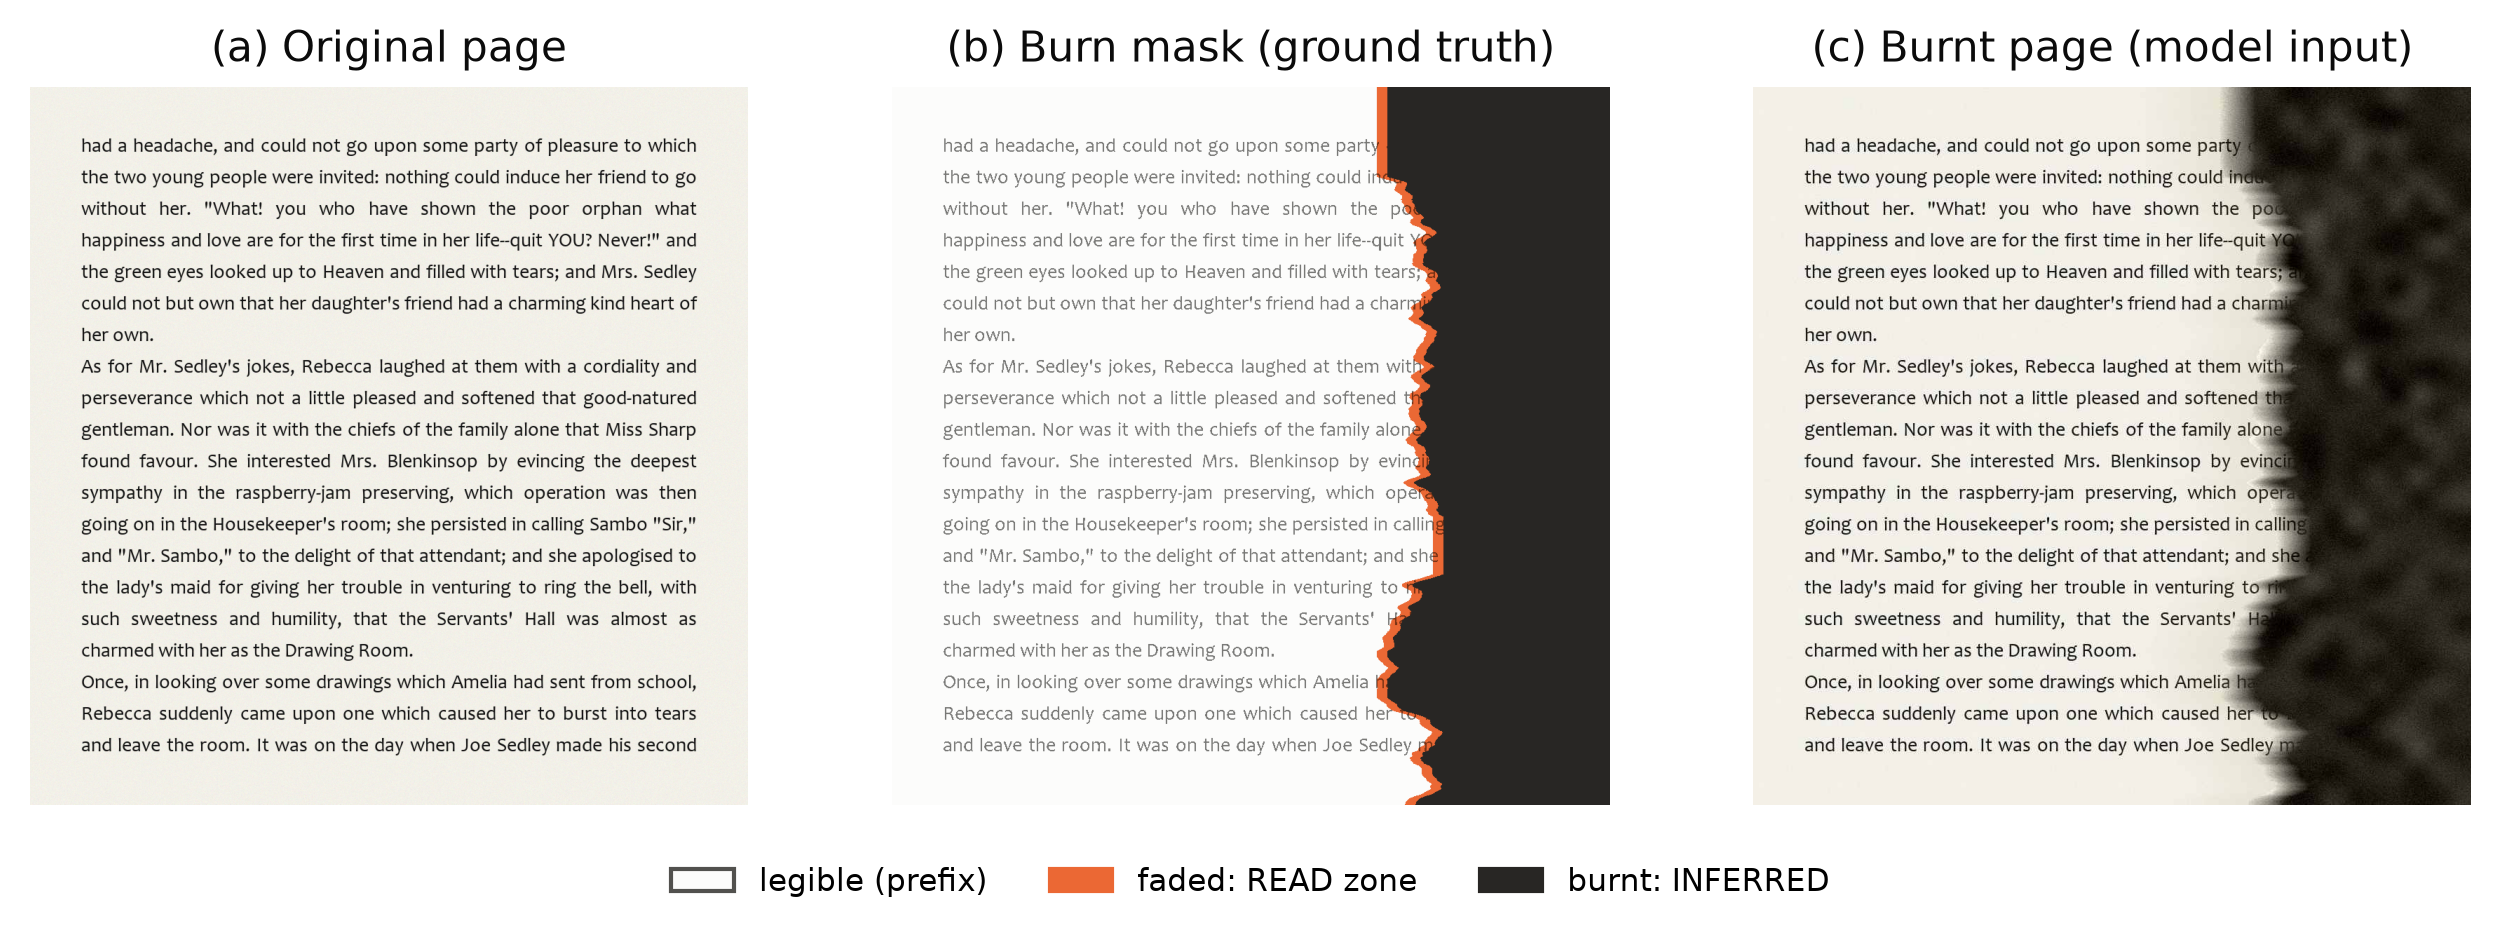
\includegraphics[width=\linewidth]{fig_pipeline.png}
\caption{A held-out synthetic page. (a) Original page. (b) Ground-truth burn mask: legible text
(white), faded band with visible strokes (orange, the \READ\ zone) and charred region (black, the
\INF\ zone). (c) The burnt page given to the model.}
\label{fig:pipeline}
\end{figure}

\section{Objectives}
\begin{enumerate}[leftmargin=2em,itemsep=1pt]
\item Generate realistic side-burnt pages with an exact label for every character: legible,
faded-but-visible, or burnt.
\item Build a multimodal model that reads the faded strokes and uses the context for the rest.
\item Keep every predicted ending inside the physical space destroyed by the burn.
\item Evaluate the \READ\ and \INF\ parts separately, against ablations and an external baseline,
with significance tests and calibration analysis.
\item Provide a working demo that presents suggestions as hypotheses.
\end{enumerate}

\section{Related work}
Pythia~\cite{assael2019pythia} and Ithaca~\cite{assael2022ithaca} restore missing characters of
ancient inscriptions from the transcribed text alone and report ranked hypotheses; we add the
image and keep the ranked output. Virtual unwrapping~\cite{seales2016engedi} recovers ink that is
physically present but invisible; our setting is an ordinary photograph. For recognition we use
CTC~\cite{graves2006ctc}; TrOCR~\cite{li2023trocr} and Tesseract~\cite{smith2007tesseract} serve as
OCR candidates for the external baseline. The model builds on T5~\cite{raffel2020t5}, whose
span-filling pretraining matches our task, ResNet~\cite{he2016resnet}, zero-initialised gated
cross-attention from Flamingo~\cite{alayrac2022flamingo} and a CLIP-style~\cite{radford2021clip}
contrastive term. Qwen2.5~\cite{qwen2024} is the language model of the baseline. Confidence is
evaluated with ECE~\cite{naeini2015ece} and Platt scaling~\cite{platt1999}, following
Guo et al.~\cite{guo2017calibration}, and differences with the paired
bootstrap~\cite{efron1993bootstrap}. We found no prior work that treats side-burnt printed lines
as a vision--language completion problem, separates the visible from the destroyed part in
evaluation, and enforces a calibrated physical length bound during decoding; these are the
contributions of this project.

% =====================================================================
\chapter{Methodology}\label{ch:method}
% =====================================================================
\section{Overview}
The method has five steps:
\begin{enumerate}[leftmargin=2em,itemsep=1pt]
\item \textbf{Generate} book pages and burn their right side with randomised parameters.
\item \textbf{Label} every character of each severed line as prefix, \READ\ or \INF.
\item \textbf{Encode} the surviving text with T5 and a crop of the burn edge with a ResNet, and fuse
them with gated cross-attention.
\item \textbf{Decode} the missing ending with beam search under a calibrated length bound.
\item \textbf{Evaluate} the \READ\ and \INF\ parts separately on books never seen in training.
\end{enumerate}

\section{Synthetic data generation}
\textbf{Rendering.} Text comes from 57 Project Gutenberg~\cite{gutenberg} books, split \emph{by book}
into training, validation and test sets (Table~\ref{tab:data}). Pages are rendered at
$1024\times1024$ pixels in one of 16 fonts with random size, margins, line spacing, paper colour
and ink darkness, with paragraph indents, justification and hyphenation. The renderer stores the
horizontal extent of every character.

\textbf{Burn model.} A jagged boundary $b(y)$ removes 15--30\% of the page width. Charring is an
opacity layer that rises across a fade band of random width $T\in[30,80]$\,px with a random curve
$\gamma\in[0.6,1.8]$:
\begin{equation}
\alpha(x,y)=\operatorname{clip}\!\left(\frac{x-(b(y)-T)}{T},\,0,\,1\right)^{\gamma}.
\end{equation}
A scorch halo, blotchy texture, noise, blur and JPEG compression are added at random.

\textbf{Labels.} With $\alpha_c$ the opacity at the centre of character $c$:
\begin{equation}
c\in\begin{cases}
\text{prefix} & \alpha_c<0.5,\\
\READ & 0.5\le\alpha_c<0.8 \text{ (leading characters only)},\\
\INF & \text{otherwise.}
\end{cases}
\end{equation}
The model input is the surviving text and a $128\times256$ crop centred on the burn edge
(Figure~\ref{fig:linezoom}).

\begin{table}[H]
\centering\small
\caption{Dataset (v3), split by book.}\label{tab:data}
\begin{tabular}{@{}lccc@{}}
\toprule
Split & Books & Pages & Severed lines\\
\midrule
Training & 47 & 5{,}000 & 98{,}176\\
Validation & 4 & 200 & 3{,}961\\
Test & 6 & 300 & 6{,}145\\
\bottomrule
\end{tabular}
\end{table}

\begin{figure}[H]
\centering
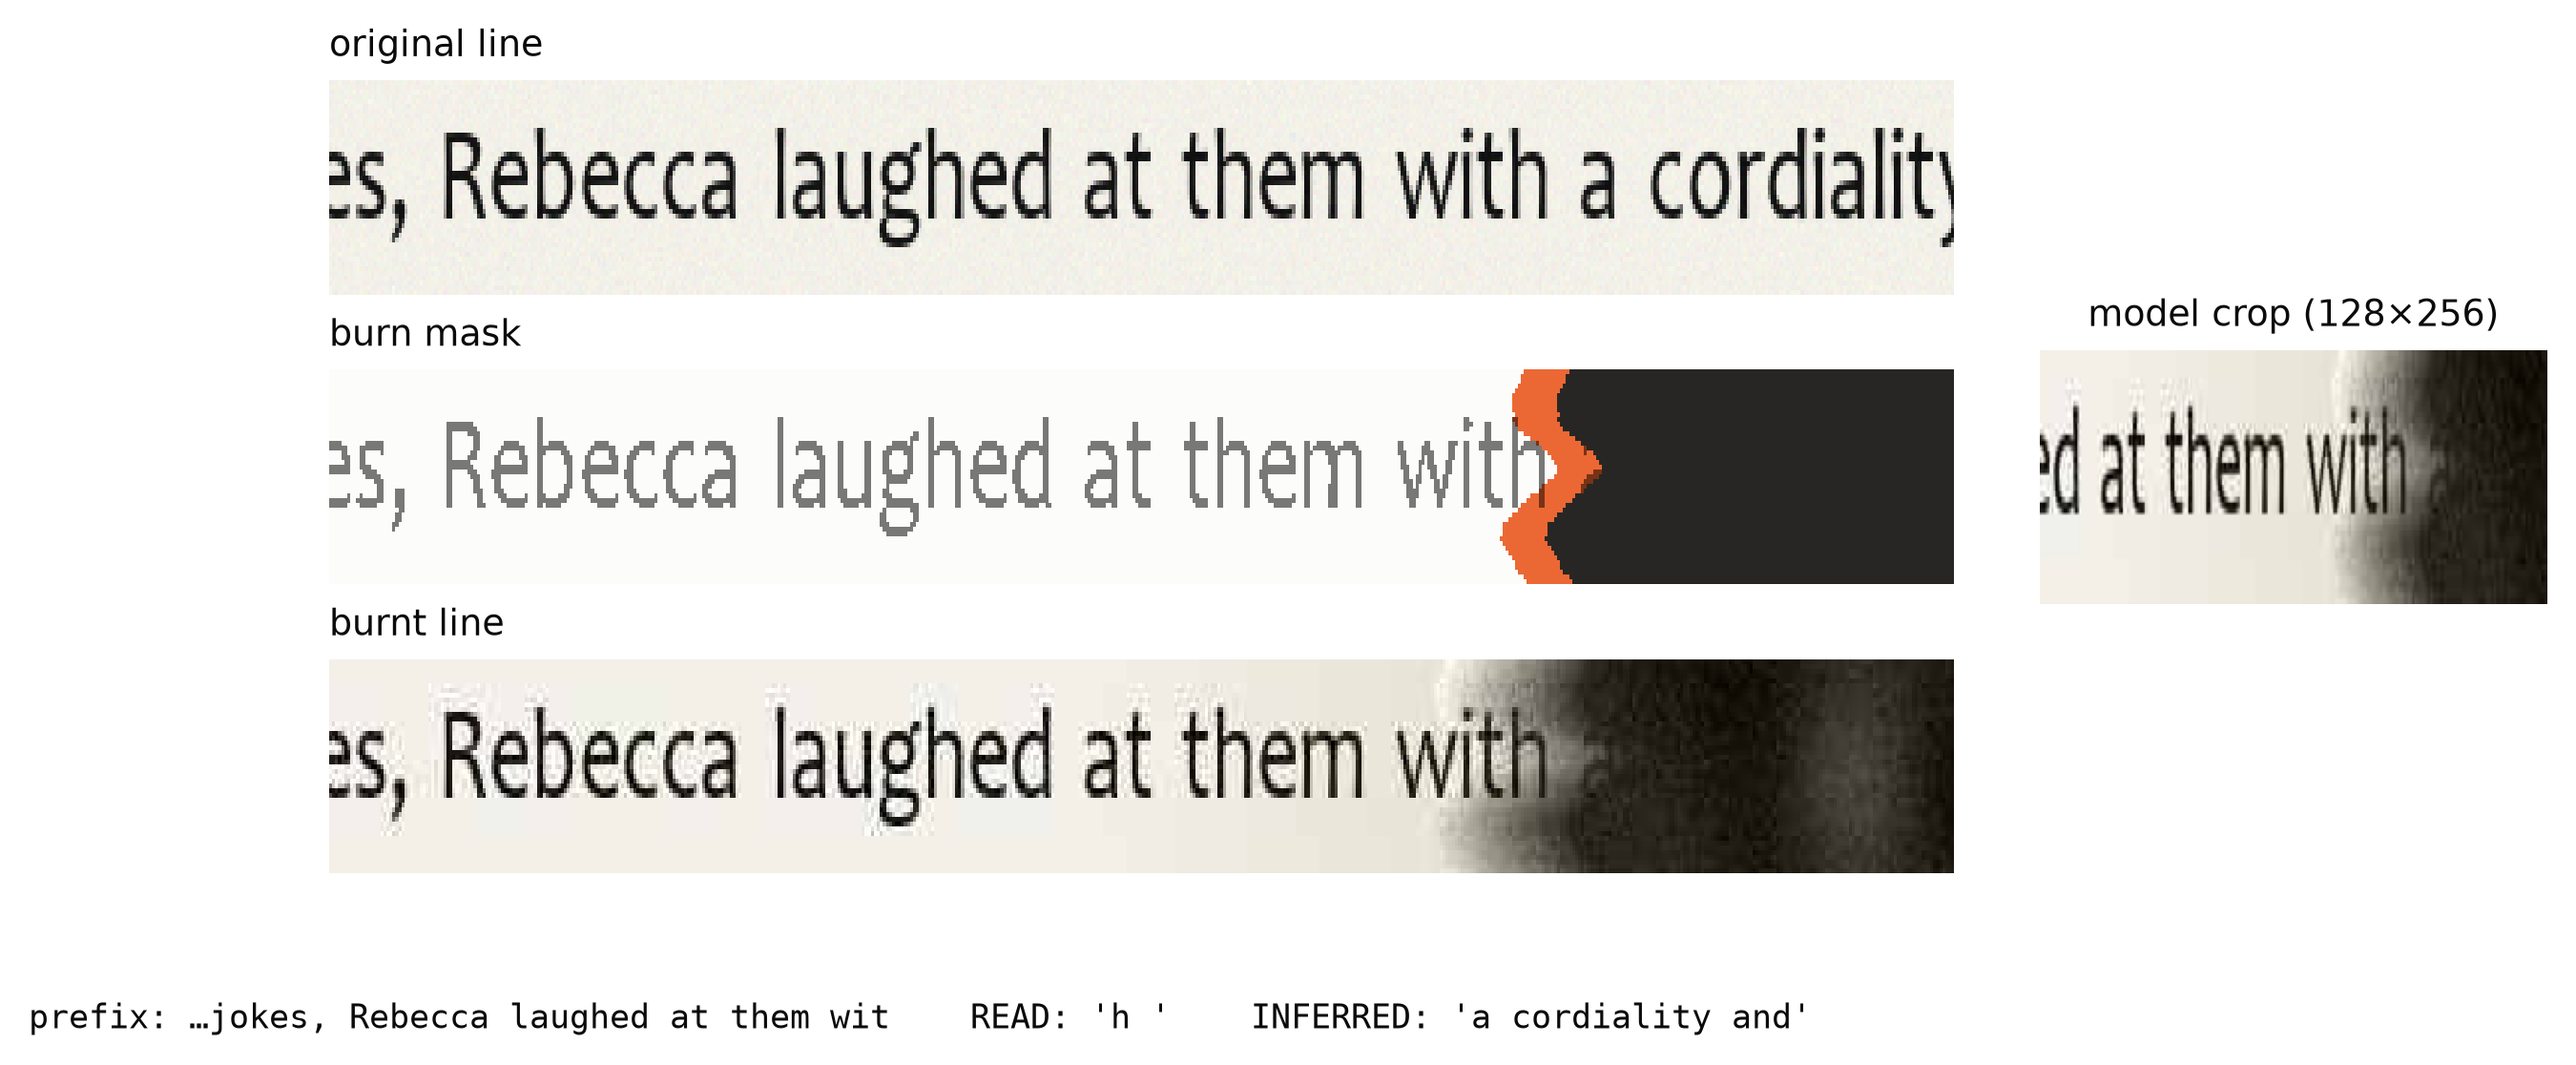
\includegraphics[width=\linewidth]{fig_line_zoom.png}
\caption{One severed line: original, ground-truth mask, burnt line and the $128\times256$ crop the
model sees, with the surviving prefix, the \READ\ part and the \INF\ part of the target.}
\label{fig:linezoom}
\end{figure}

\section{Model architecture}
Figure~\ref{fig:arch} shows the model.

\begin{figure}[H]
\centering
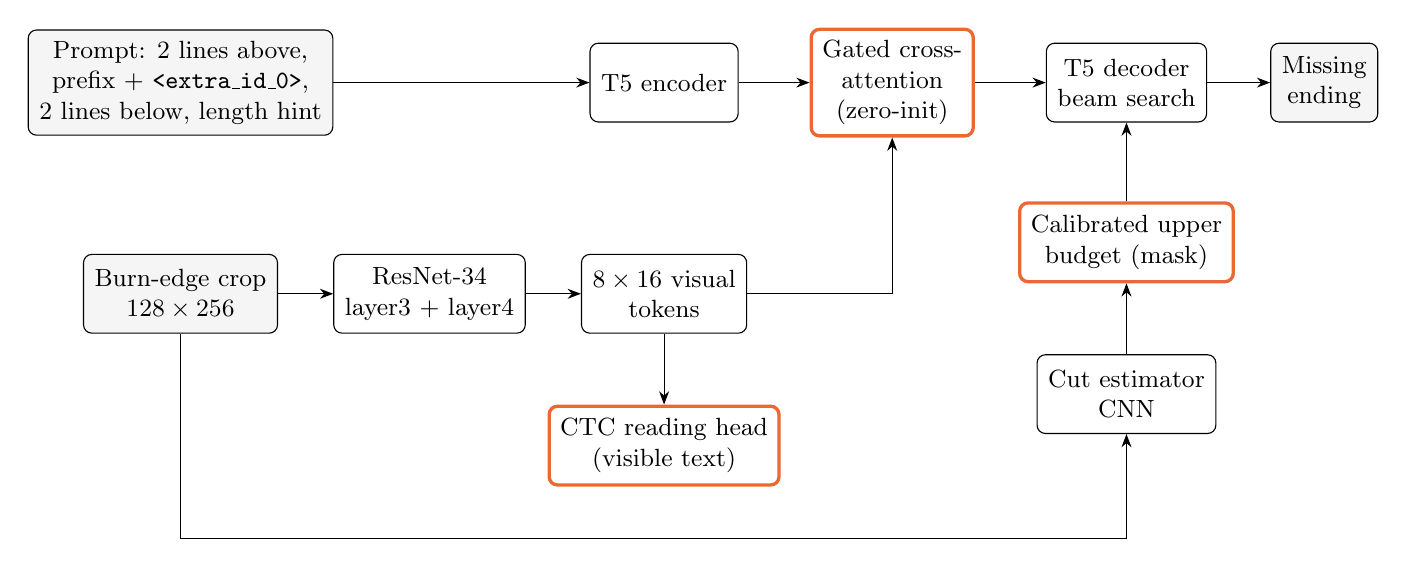
\begin{tikzpicture}[font=\small,>=Stealth,
  box/.style={draw,rounded corners=3pt,align=center,minimum height=1.0cm,inner sep=4pt,fill=white},
  io/.style={box,fill=black!4},
  ours/.style={box,draw=corange,very thick}]
\node[io] (crop) {Burn-edge crop\\$128\times256$};
\node[box,right=0.7cm of crop] (resnet) {ResNet-34\\layer3 + layer4};
\node[box,right=0.7cm of resnet] (tok) {$8\times16$ visual\\tokens};
\node[ours,below=0.9cm of tok] (ctc) {CTC reading head\\(visible text)};
\node[io,above=1.5cm of crop] (prompt) {Prompt: 2 lines above,\\prefix $+$ \texttt{<extra\_id\_0>},\\2 lines below, length hint};
\node[box] (enc) at (prompt -| tok) {T5 encoder};
\node[ours,right=0.9cm of enc] (fuse) {Gated cross-\\attention\\(zero-init)};
\node[box,right=0.9cm of fuse] (dec) {T5 decoder\\beam search};
\node[ours,below=1.0cm of dec] (bud) {Calibrated upper\\budget (mask)};
\node[box,below=0.9cm of bud] (cut) {Cut estimator\\CNN};
\node[io,right=0.8cm of dec] (out) {Missing\\ending};
\draw[->] (crop) -- (resnet); \draw[->] (resnet) -- (tok);
\draw[->] (tok) -- (ctc);
\draw[->] (prompt) -- (enc); \draw[->] (enc) -- (fuse);
\draw[->] (tok.east) -| (fuse.south);
\draw[->] (fuse) -- (dec); \draw[->] (dec) -- (out);
\draw[->] (cut) -- (bud); \draw[->] (bud) -- (dec);
\draw[->] (crop.south) |- ++(0,-2.6) -| (cut.south);
\end{tikzpicture}
\caption{Model overview. Components outlined in orange are additions made in this project on top
of a T5 + ResNet baseline.}
\label{fig:arch}
\end{figure}

\textbf{Text encoder.} The prompt holds the surviving prefixes of two lines above and two below,
the current prefix followed by the T5 sentinel \texttt{<extra\_id\_0>}, and an estimate of the
number of missing characters. We use t5-small (60\,M parameters) and t5-base (220\,M).

\textbf{Image encoder.} A ResNet-34 encodes the crop; features of its last two stages are combined
into an $8\times16$ grid of visual tokens $V$, about one character per token.

\textbf{Gated fusion.} Each T5 encoder state $h$ attends to the visual tokens:
\begin{equation}
h' = h + \tanh(g)\cdot\operatorname{MHA}(h, V, V),\qquad g\ \text{initialised to } 0,
\end{equation}
so training starts from the unchanged pretrained T5 and the image is blended in only as far as it
helps.

\textbf{Reading head.} A CTC head on the visual tokens transcribes the text visible in the crop. It
forces the vision encoder to learn glyphs and gives the demo a reading that does not depend on the
language model.

\section{Training objective}
The loss combines generation, reading and a contrastive alignment term:
\begin{equation}
\mathcal{L} = \mathcal{L}_{\text{gen}} + \lambda_{\text{read}}\,\mathcal{L}_{\text{CTC}}
+ \lambda_{c}\,\mathcal{L}_{\text{con}},\qquad \lambda_{\text{read}}=0.3,\ \lambda_c=0.2,
\end{equation}
where $\mathcal{L}_{\text{gen}}$ is the cross-entropy of the target ending, $\mathcal{L}_{\text{CTC}}$
the CTC loss of the visible text, and $\mathcal{L}_{\text{con}}$ aligns visual and text features
\emph{only on \READ\ characters}: aligning image features with text that is not in the image would
teach the encoder to hallucinate. The text-only baseline drops the last two terms.

\section{Calibrated length bound}
The missing length is estimated from geometry: $\hat n = (x_{\text{margin}} - x_{\text{cut}})/\bar w$,
the gap from the cut to the right text margin divided by the mean glyph width of the prefix. The
original decoder only penalised endings longer than $\hat n + 2$; that rule cut off 7.6\% of
\emph{correct} endings yet still let models run 7 characters past $\hat n$. We replaced it with:
\begin{enumerate}[leftmargin=2em,itemsep=1pt]
\item a small CNN that predicts $x_{\text{cut}}$ from the crop (error 0.96\,px, against 7.3\,px for
the fixed offset used before);
\item an upper bound $u = 1.139\,\hat n + 1$, calibrated on validation lines so that 99\% of true
endings fit (98.8\% on test);
\item a logits mask in beam search that removes every token that would make the decoded ending
longer than $u$, so no output can exceed the bound.
\end{enumerate}

\section{Evaluation protocol}
All systems are scored on the same 6{,}145 test lines with the same beam search ($k=5$) and the same
bound (Table~\ref{tab:metrics}). Systems: an empty prediction, zero-shot t5-small, a \textbf{text-only}
model trained on the same data without the image, the \textbf{full} model, the full model with a
blank or mismatched image (ablations), and an external \textbf{OCR + LLM} baseline
(Section~\ref{sec:baseline}). Differences use a paired bootstrap ($B=1000$).

\begin{table}[H]
\centering\small
\caption{Evaluation metrics.}\label{tab:metrics}
\begin{tabularx}{\linewidth}{@{}lX@{}}
\toprule
Metric & What it measures\\
\midrule
\READ\ accuracy & top-1 prediction starts with exactly the \READ\ characters\\
\INF\ CER & character error rate on the burnt rest of the target\\
CER, EM & whole target: character error rate and exact match\\
EM@5, 1st word@5 & the truth is among the 5 ranked hypotheses\\
bits/char & $-\log_2 p(\text{truth})$ per character; lower means the truth is more likely\\
AUROC, ECE & whether first-word confidence separates right from wrong, and its calibration\\
overlong & top-1 more than 3 characters longer than the true ending\\
\bottomrule
\end{tabularx}
\end{table}

% =====================================================================
\chapter{Implementation}\label{ch:impl}
% =====================================================================
\section{Training procedure}
Training has two stages. In stage 1 (one epoch) T5 is frozen and only the vision encoder, fusion and
heads learn. In stage 2 all parameters are fine-tuned with per-group learning rates. Mixed precision
(bfloat16) and gradient clipping are used throughout, and the checkpoint with the lowest validation
CER is kept (Table~\ref{tab:hparams}, Figure~\ref{fig:training}).

\begin{table}[H]
\centering\small
\caption{Training settings.}\label{tab:hparams}
\begin{tabular}{@{}ll@{}}
\toprule
Setting & Value\\
\midrule
Batch size & 16\\
Epochs & 5 (t5-small), 3 (t5-base, gradient checkpointing)\\
Learning rates (stage 2) & T5 and ResNet $1\times10^{-5}$; fusion and heads $5\times10^{-5}$\\
Stage-1 learning rate & $1\times10^{-4}$ (adapters only)\\
Weight decay, gradient clip & $10^{-4}$, 1.0\\
Max.\ prompt / target length & 256 / 32 tokens\\
Time per epoch & $\approx$21 min (t5-small), $\approx$70 min (t5-base)\\
Peak GPU memory & 4.6\,GiB (t5-base with vision encoder)\\
\bottomrule
\end{tabular}
\end{table}

\begin{figure}[H]
\centering
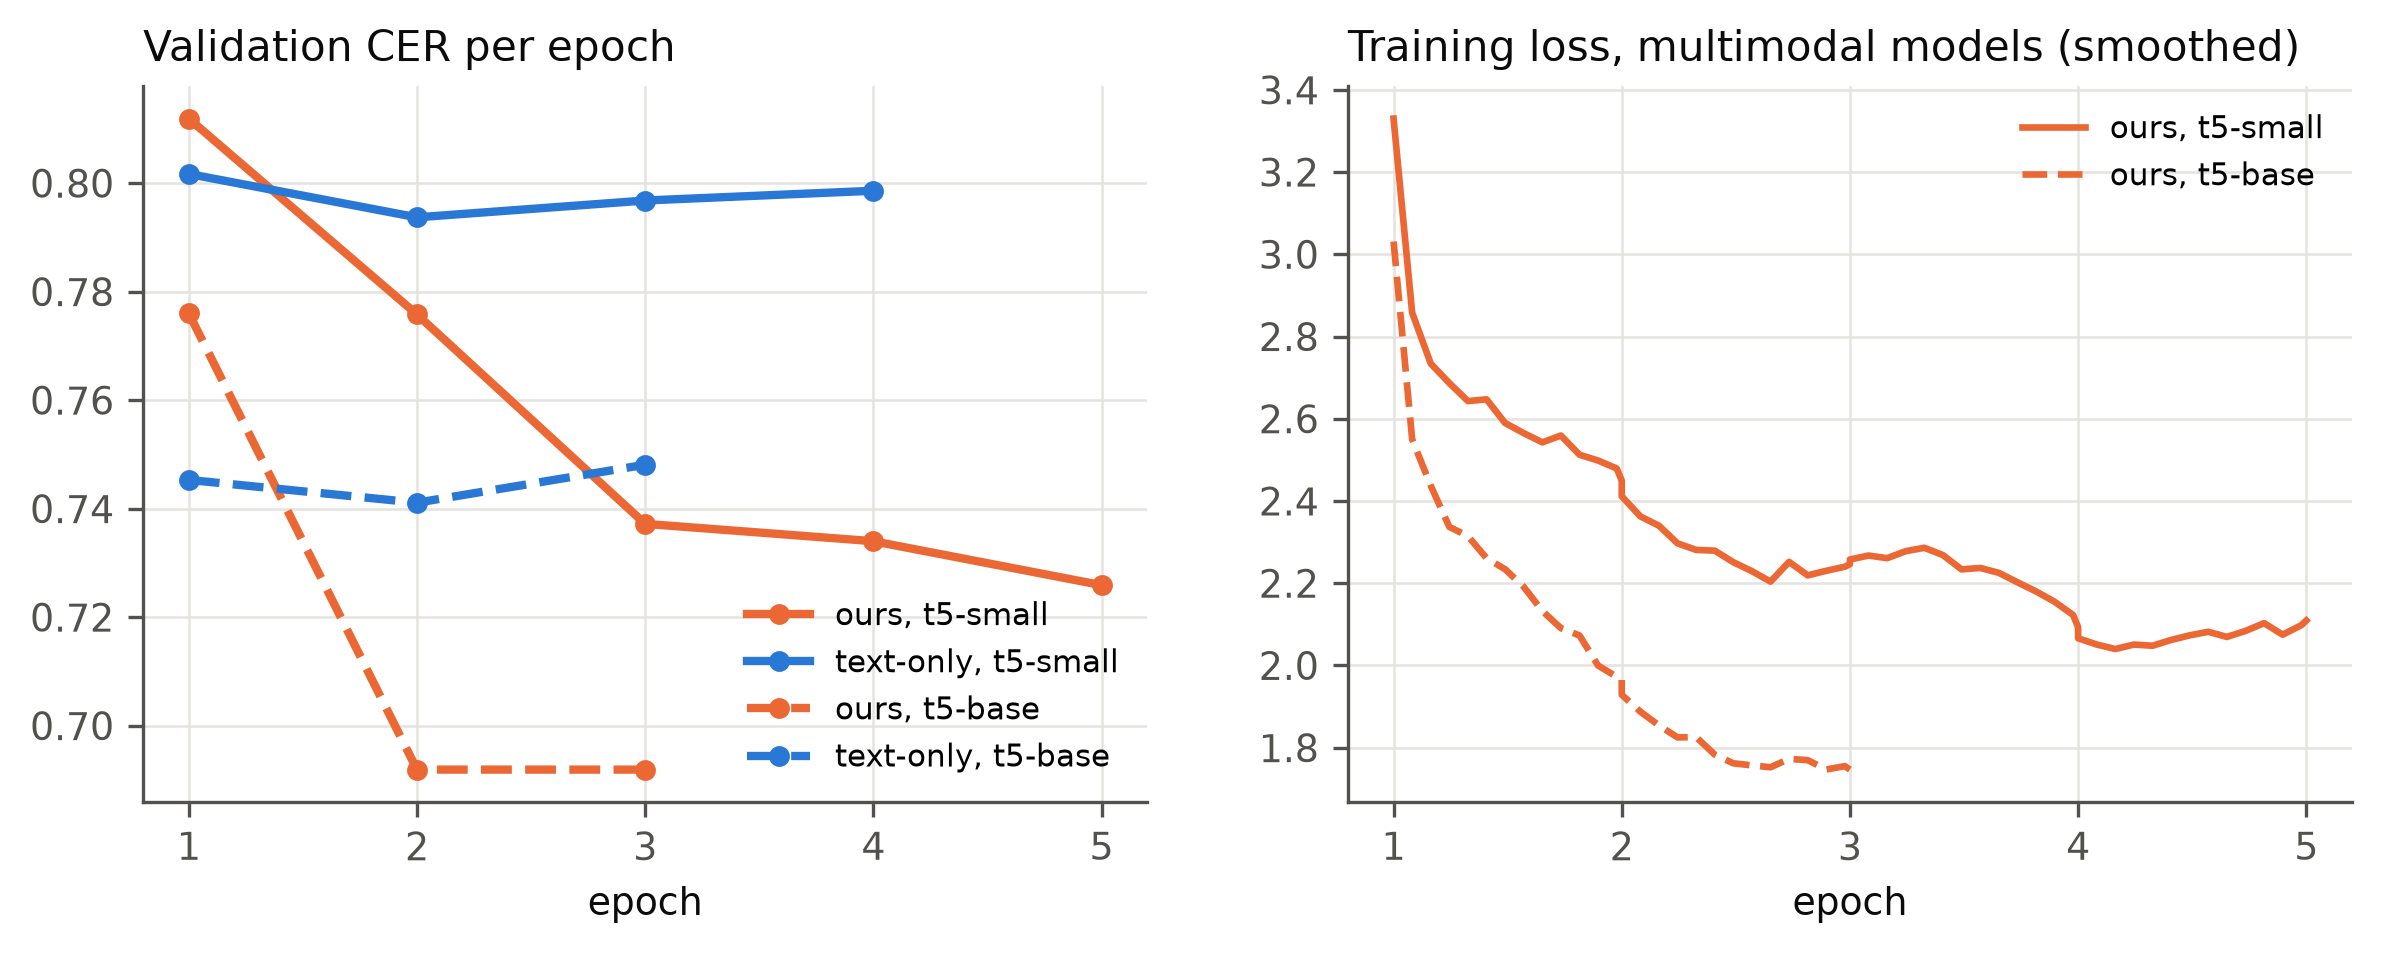
\includegraphics[width=\linewidth]{fig_training.png}
\caption{Left: validation CER after each epoch (800 lines). Right: smoothed training loss of the
multimodal models; the drop at epoch 2 is where stage 2 unfreezes T5.}
\label{fig:training}
\end{figure}

\section{Software structure}
Preprocessing is defined once and shared by training, evaluation and inference:
\begin{itemize}[leftmargin=2em,itemsep=1pt]
\item \texttt{line\_data.py}: page rendering, burns, crops, prompts, \READ/\INF\ split, length estimate;
\item \texttt{model.py}: the restorer, fusion, CTC head, cut estimator and the length-bound logits mask;
\item \texttt{train.py}: the two-stage trainer;
\item \texttt{scripts/evaluate\_lines.py}: evaluation, bootstrap tests and calibration;
\item \texttt{scripts/baseline\_ocr\_llm.py}: the external OCR + LLM baseline;
\item \texttt{inference/}, \texttt{api/}: page-level burn detector, restoration engine and FastAPI web service;
\item \texttt{tests/}: 115 unit and integration tests.
\end{itemize}

\section{Page-level pipeline and demo}
For a full page, a burn detector finds the burn front from normalised darkness and splits the page
into lines; on 120 synthetic test pages it finds 99.6\% of severed lines and places the burn edge
within 5\,px on average. The user pastes the surviving text, and the web interface shows for each
severed line the top suggestion, alternatives, the vision-only reading and the length estimate,
stating that suggestions are hypotheses (Figure~\ref{fig:ui}).

\begin{figure}[H]
\centering
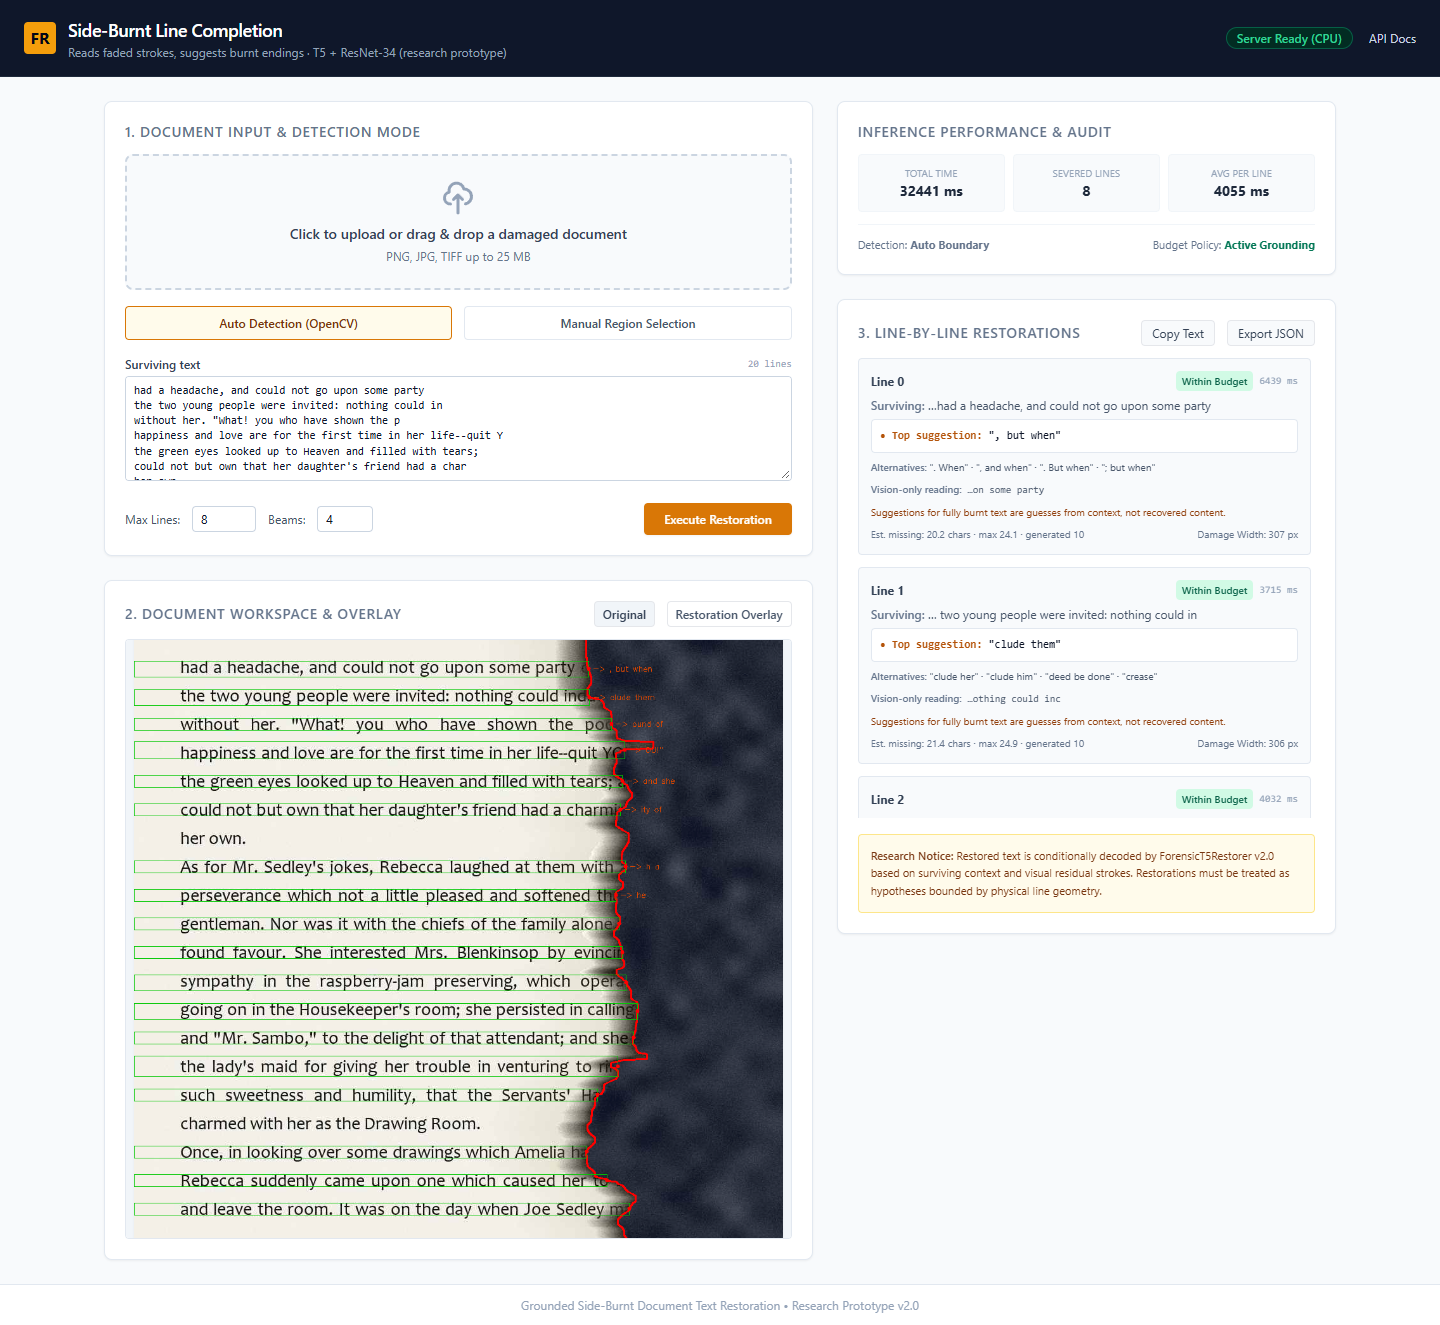
\includegraphics[width=0.8\linewidth]{fig_ui_demo.png}
\caption{The web demo on a held-out synthetic page (pasted text is the generator's transcription).}
\label{fig:ui}
\end{figure}

\section{Hardware and software}
All experiments ran on one NVIDIA GeForce RTX 4050 Laptop GPU (6\,GB) under Windows 11, with
Python 3, PyTorch 2 (CUDA 12.6) and Hugging Face Transformers 4.57; OpenCV, Pillow and NumPy for
images; Matplotlib for plots; FastAPI and Uvicorn for the demo; pytest and git for testing and
versioning. Pretrained models: T5-small, T5-base, ResNet-34 (ImageNet), and TrOCR and
Qwen2.5-1.5B for the baseline.

% =====================================================================
\chapter{Results and Outcomes}\label{ch:results}
% =====================================================================
All numbers are on the 6{,}145 test lines from books never seen in training.

\section{Main results}
\begin{table}[H]
\centering\small\setlength{\tabcolsep}{4pt}
\caption{Main results. $\uparrow$ higher is better, $\downarrow$ lower is better.}
\label{tab:main}
\resizebox{\linewidth}{!}{%
\begin{tabular}{@{}lcccccccc@{}}
\toprule
System & \READ\ acc$\uparrow$ & \INF\ CER$\downarrow$ & CER$\downarrow$ & EM$\uparrow$ & EM@5$\uparrow$ & 1st word$\uparrow$ & bits/char$\downarrow$ & overlong$\downarrow$\\
\midrule
Empty prediction & 0 & 1.000 & 1.000 & 0 & 0 & 0 & -- & 0\\
Zero-shot t5-small & 0.113 & 1.040 & 1.015 & 0.001 & 0.002 & 0.060 & 4.27 & 44.8\%\\
Text-only, t5-small & 0.232 & 0.815 & 0.775 & 0.037 & 0.063 & 0.166 & 1.85 & 1.8\%\\
\textbf{Ours, t5-small} & \textbf{0.700} & 0.768 & 0.699 & 0.069 & 0.118 & 0.401 & 1.57 & 1.9\%\\
Text-only, t5-base & 0.361 & 0.741 & 0.702 & 0.078 & 0.132 & 0.293 & 1.44 & 2.7\%\\
\textbf{Ours, t5-base} & 0.660 & \textbf{0.717} & \textbf{0.656} & \textbf{0.103} & \textbf{0.174} & \textbf{0.418} & \textbf{1.31} & 2.4\%\\
\bottomrule
\end{tabular}}
\end{table}

Adding the image raises \READ\ accuracy from 0.23 to 0.70 with t5-small and from 0.36 to 0.66 with
t5-base; all differences to the text-only model of the same size are significant ($p<0.001$). The
\INF\ CER improves much less (0.815$\to$0.768 and 0.741$\to$0.717). The larger language model helps
the guessing: t5-base lowers bits/char from 1.57 to 1.31 and \INF\ CER from 0.768 to 0.717.
Figure~\ref{fig:qual} shows test lines: the full model reads the faded start of the ending
(\emph{he}, \emph{iving}, \emph{r.}) where the text-only model guesses wrong (\emph{hat},
\emph{oyal}, \emph{s.}); after the visible characters both models guess.

\begin{figure}[H]
\centering
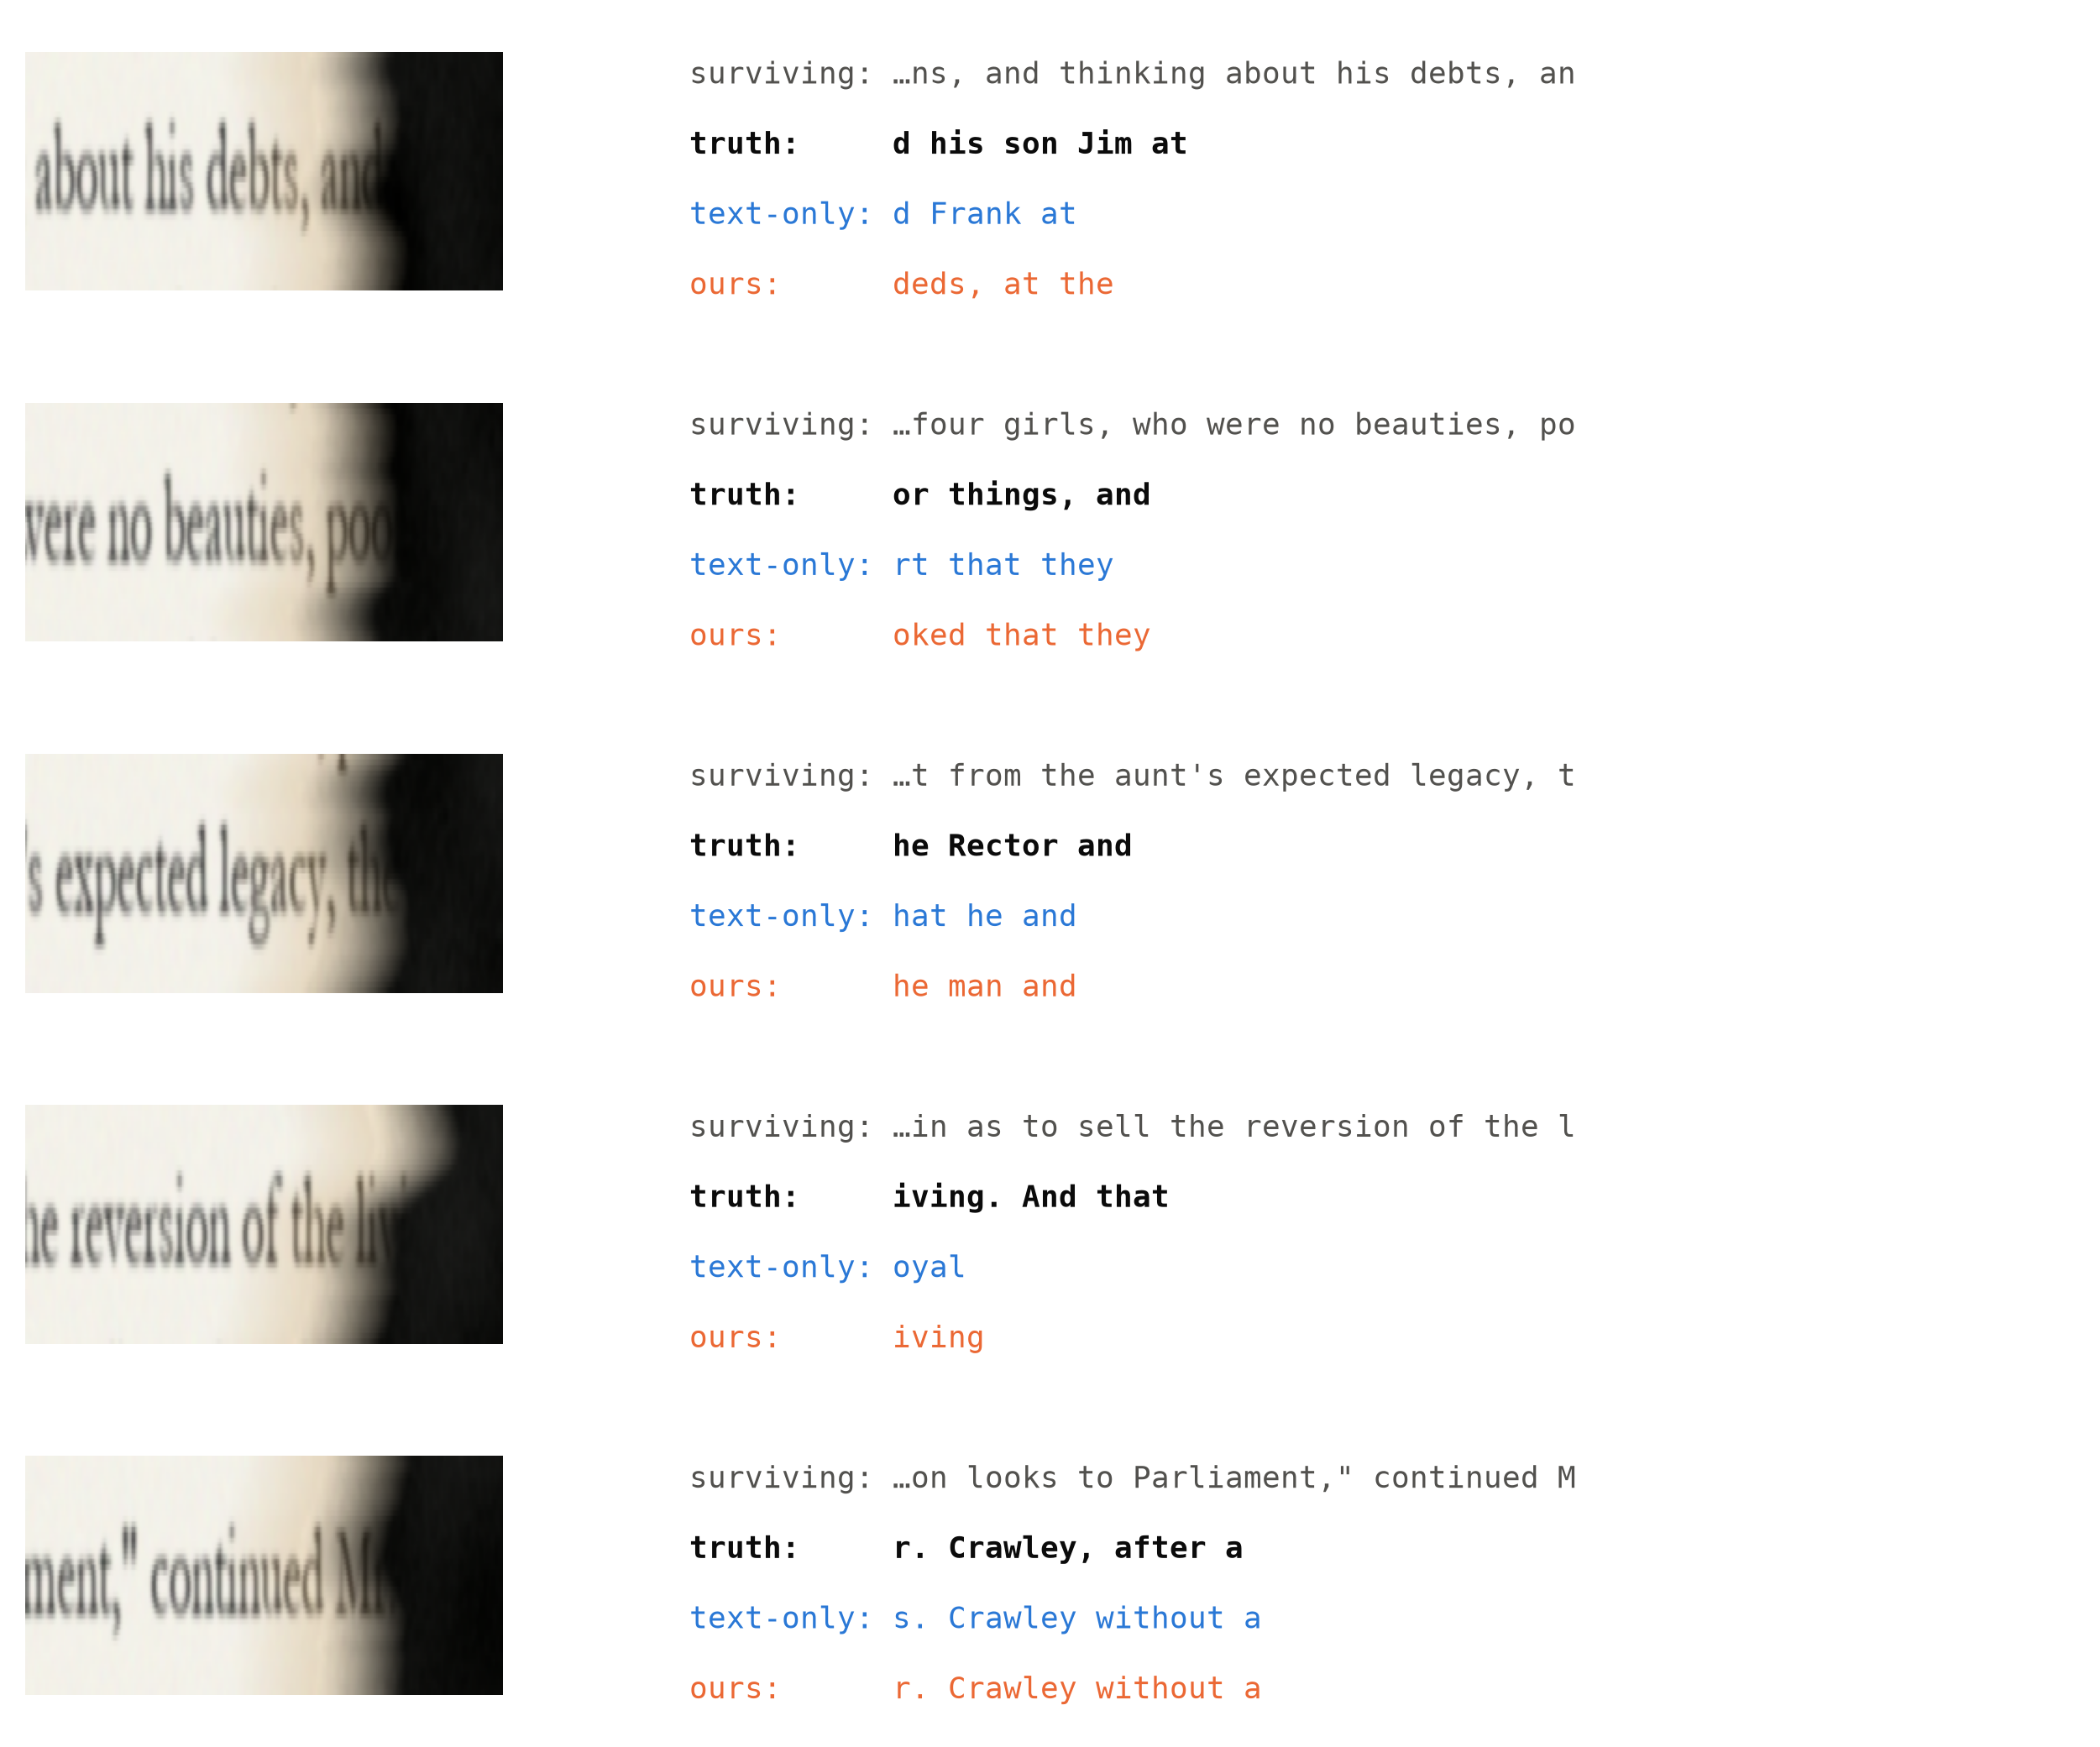
\includegraphics[width=0.9\linewidth]{fig_qualitative.png}
\caption{Test lines: input crop, surviving text, truth, text-only prediction (blue) and our
prediction (orange), t5-base.}
\label{fig:qual}
\end{figure}

\section{Ablations: does the model use the image?}\label{sec:ablation}
With a blank image, \READ\ accuracy falls from 0.70 to 0.16 (t5-small); with the crop of a
different line it falls to 0.07, below the text-only model, because the model reads the wrong
strokes (Figure~\ref{fig:ablation}). The CTC head alone transcribes the visible text with a CER of
0.03. For the burnt part, blanking the image leaves \INF\ CER unchanged for t5-small (0.823 vs.\
0.827, not significant). \textbf{The image reads faded characters; it does not recover burnt text.}

\begin{figure}[H]
\centering
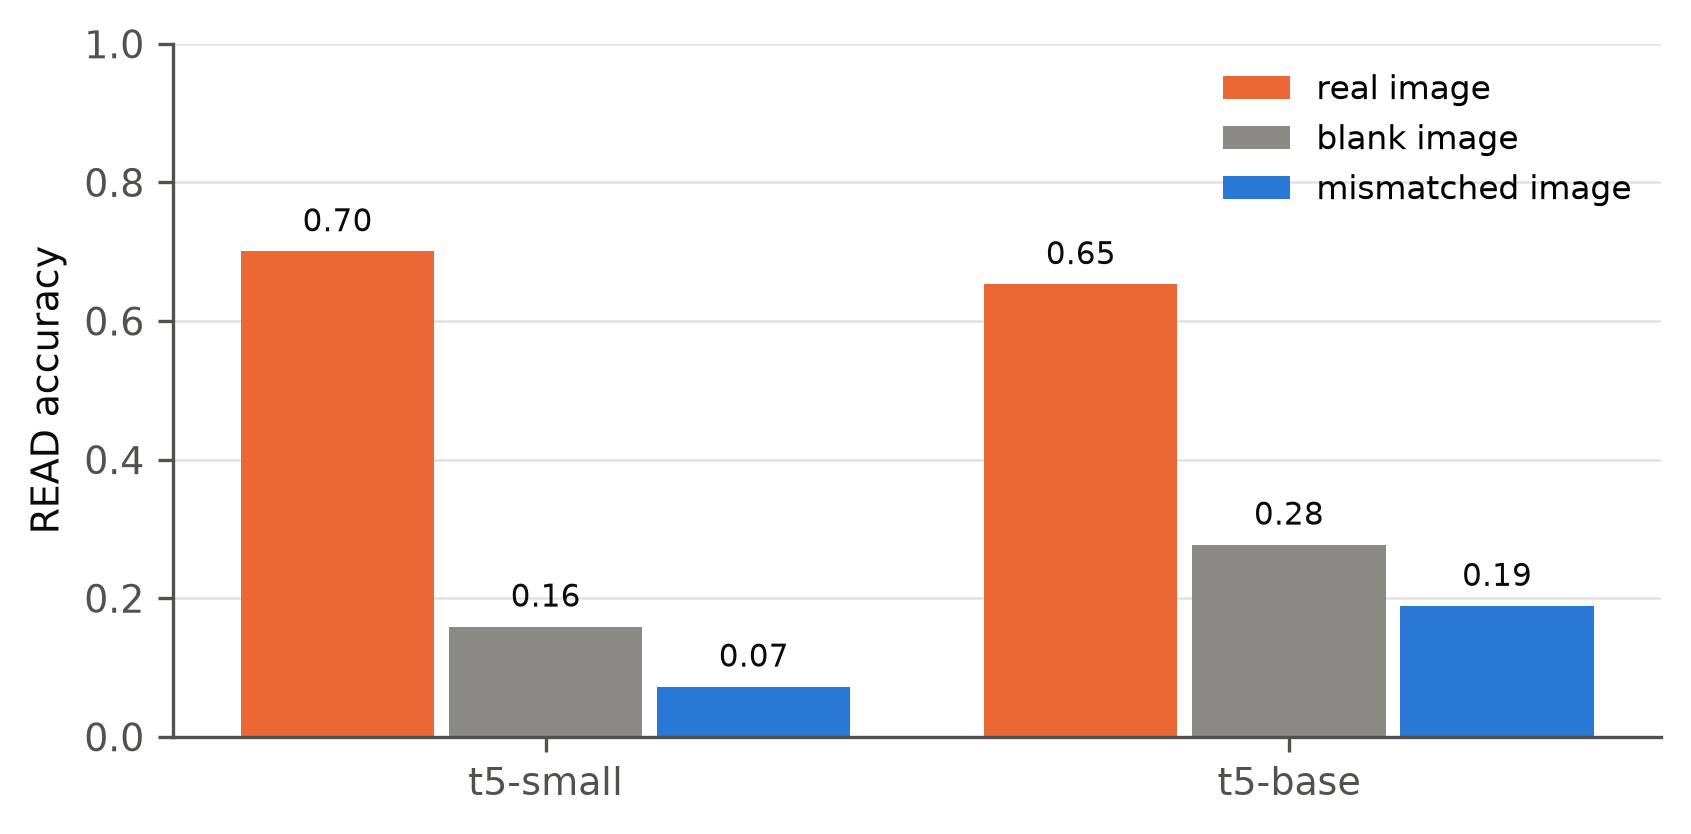
\includegraphics[width=0.65\linewidth]{fig_ablation.png}
\caption{\READ\ accuracy with the real crop, a blank crop and the crop of a different line.}
\label{fig:ablation}
\end{figure}

\section{Effect of the calibrated length bound}
\begin{table}[H]
\centering\small
\caption{Old length rule against the calibrated upper bound; same checkpoints and test lines.}
\label{tab:budget}
\resizebox{\linewidth}{!}{%
\begin{tabular}{@{}llccccc@{}}
\toprule
System & Length rule & CER$\downarrow$ & \INF\ CER$\downarrow$ & EM$\uparrow$ & overlong$\downarrow$ & exceeds bound$\downarrow$\\
\midrule
\multirow{2}{*}{Text-only, t5-small} & old & 0.810 & 0.853 & 0.029 & 8.7\% & 8.4\%\\
 & calibrated & \textbf{0.775} & \textbf{0.815} & \textbf{0.037} & \textbf{1.8\%} & \textbf{0\%}\\
\multirow{2}{*}{Ours, t5-small} & old & 0.755 & 0.827 & 0.048 & 12.2\% & 11.7\%\\
 & calibrated & \textbf{0.699} & \textbf{0.768} & \textbf{0.069} & \textbf{1.9\%} & \textbf{0\%}\\
\multirow{2}{*}{Text-only, t5-base} & old & 0.795 & 0.841 & 0.052 & 20.4\% & 20.1\%\\
 & calibrated & \textbf{0.702} & \textbf{0.741} & \textbf{0.078} & \textbf{2.7\%} & \textbf{0\%}\\
\multirow{2}{*}{Ours, t5-base} & old & 0.744 & 0.810 & 0.068 & 18.7\% & 18.3\%\\
 & calibrated & \textbf{0.656} & \textbf{0.717} & \textbf{0.103} & \textbf{2.4\%} & \textbf{0\%}\\
\bottomrule
\end{tabular}}
\end{table}

The calibrated bound was the largest single gain on the guessed part (Table~\ref{tab:budget}):
overlong endings fall from 9--20\% to about 2\%, and \INF\ CER improves by 0.04--0.10 for every
model ($p<0.001$). Putting the calibrated estimate into the prompt as well (retraining all four
models) changed CER by at most 0.008, so the original checkpoints were kept.

\section{Confidence}
The first-word confidence separates right from wrong answers (Table~\ref{tab:calib}): in its most
confident quarter, our t5-base model is right 88\% of the time, against 70\% for the text-only
model. The raw confidence is already calibrated (ECE 0.03, Figure~\ref{fig:reliab}); Platt scaling
fitted on the validation books made it worse on the test books, so the demo shows the raw value.

\begin{table}[H]
\centering\small
\caption{Confidence of the first word: separation (AUROC), accuracy in the most confident 25\% of
lines, and calibration (ECE).}
\label{tab:calib}
\begin{tabular}{@{}lcccc@{}}
\toprule
System & AUROC$\uparrow$ & Acc.\ top 25\%$\uparrow$ & ECE raw$\downarrow$ & ECE Platt$\downarrow$\\
\midrule
Text-only, t5-small & 0.841 & 0.441 & 0.017 & 0.014\\
\textbf{Ours, t5-small} & \textbf{0.896} & \textbf{0.897} & 0.037 & 0.077\\
Text-only, t5-base & 0.840 & 0.696 & 0.033 & 0.046\\
Ours, t5-base & 0.866 & 0.876 & 0.029 & 0.079\\
\bottomrule
\end{tabular}
\end{table}

\begin{figure}[H]
\centering
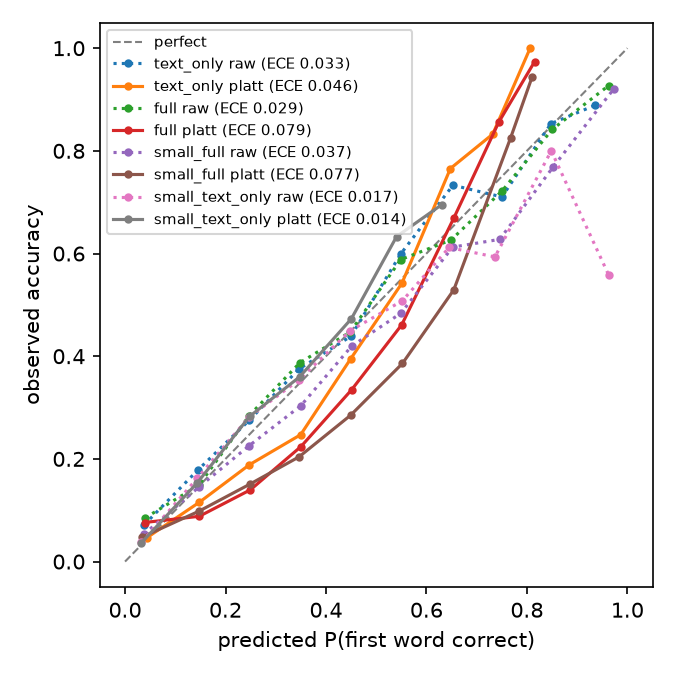
\includegraphics[width=0.45\linewidth]{fig_reliability.png}
\caption{Reliability diagram of the first-word confidence on the test books.}
\label{fig:reliab}
\end{figure}

\section{External baseline: off-the-shelf OCR + a larger language model}\label{sec:baseline}
To check the gains against strong pretrained components with no training on this task, TrOCR
(base, stage 1) reads the crop; it had the lowest error on the visible text of 150 test crops (CER
0.09, against 0.29 for Tesseract and 0.95 for TrOCR-large-printed). Whatever it reads past the known
prefix is its \READ\ guess. Qwen2.5-1.5B~\cite{qwen2024}, about seven times the size of t5-base,
continues the text with beam search; candidates are re-ranked by the likelihood of the following
line and cut to the same calibrated bound.

% Numbers from results/line_eval_baseline.json (scripts/evaluate_lines.py --extra_preds ...).
Table~\ref{tab:baseline} compares the baseline with our models on all 6,145 test lines. Every
system decodes under the same calibrated length bound, so none exceeds it.

\begin{table}[H]
\centering\small
\caption{External baseline vs.\ our models (test books, 6,145 lines). Lower is better for CER
and \INF\ CER; higher for the rest. ``First word'' is the accuracy of the first word of the
completion.}
\label{tab:baseline}
\begin{tabular}{@{}lccccc@{}}
\toprule
System & \READ\ acc & \INF\ CER & CER & First word & First word @5\
\midrule
LLM only (Qwen2.5-1.5B)          & 0.127 & 0.988 & 0.969 & 0.076 & 0.085\
OCR + LLM (TrOCR + Qwen2.5-1.5B) & 0.657 & 0.948 & 0.876 & 0.386 & 0.397\
Ours, text only (t5-base)        & 0.361 & 0.741 & 0.702 & 0.293 & 0.414\
Ours, full (t5-small)            & \textbf{0.700} & 0.768 & 0.699 & 0.401 & 0.523\
Ours, full (t5-base)             & 0.660 & \textbf{0.717} & \textbf{0.656} & \textbf{0.418} & \textbf{0.553}\
\bottomrule
\end{tabular}
\end{table}

\begin{figure}[H]
\centering
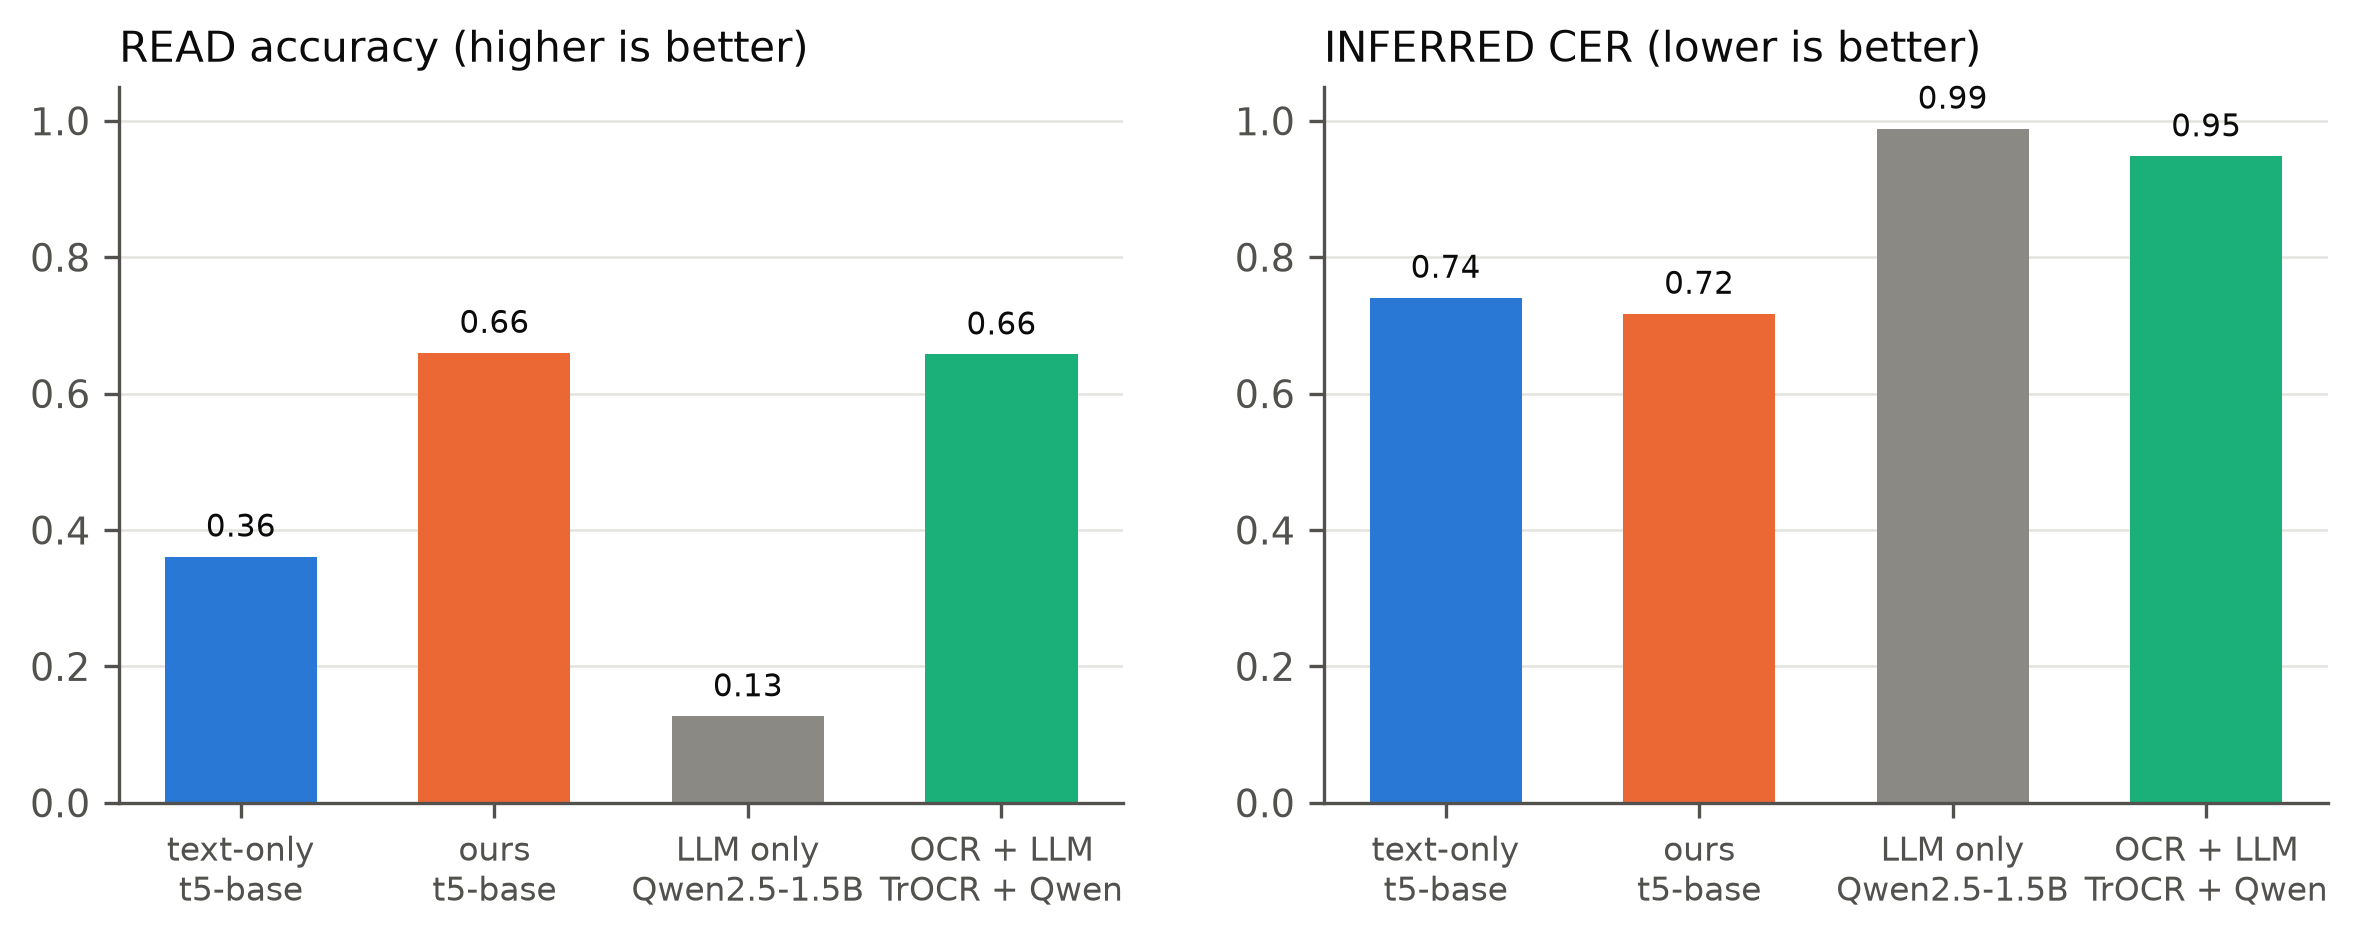
\includegraphics[width=\linewidth]{fig_baseline.png}
\caption{\READ\ accuracy and \INF\ CER of the external baseline and our models.}
\label{fig:baseline}
\end{figure}

Three results stand out (paired bootstrap, 1,000 resamples).
\begin{itemize}[leftmargin=2em,itemsep=1pt]
\item \textbf{Reading faded characters.} With OCR, the baseline reads the faded characters about
as well as our t5-base model (\READ\ accuracy 0.657 vs.\ 0.660; difference not significant,
$p=0.38$). A strong pretrained OCR model can do this step, which supports our finding that this
part of the task is reading, not guessing.
\item \textbf{Guessing the burnt part.} Our full model is far better here (\INF\ CER 0.717 vs.\
0.948, $p<0.001$; overall CER 0.656 vs.\ 0.876). Without task training, the larger LLM tends to
fill the whole available space (37.8\% of its completions are longer than the true ending, against
2.4\% for ours) and rarely reproduces the exact ending (exact match 1.4\% vs.\ 10.3\%).
\item \textbf{The image matters for the LLM too.} Without OCR the LLM gets the first word right
only 7.6\% of the time; with it, 38.6\%. Even our text-only model beats the LLM-only baseline on
every measure (CER 0.702 vs.\ 0.969).
\end{itemize}

Qwen2.5 may have seen Project Gutenberg text during pre-training, which would favour the
baseline. That it still trails our models suggests the gap comes from training on the task
(learning where lines end and how to use the length bound), not from model size.


\section{Summary of outcomes}
\begin{table}[H]
\centering\small
\caption{Main outcomes (test books).}
\label{tab:summary}
\begin{tabularx}{\linewidth}{@{}>{\raggedright\arraybackslash}X>{\raggedright\arraybackslash}p{0.22\linewidth}>{\raggedright\arraybackslash}p{0.33\linewidth}@{}}
\toprule
Question & Answer & Evidence\\
\midrule
Does the image help read faded characters? & Yes, strongly & \READ\ 0.23$\to$0.70; blank image 0.16\\
Does it recover burnt text? & No & \INF\ CER unchanged without image\\
Largest gain on the guessed part? & Calibrated length bound & overlong 9--20\%$\to$2\%\\
Does a larger LM help? & Yes, for guessing & bits/char 1.57$\to$1.31\\
Beats off-the-shelf OCR + LLM? & Yes, on the guess & \INF\ CER 0.72 vs.\ 0.95; \READ\ equal\\
Is the confidence useful? & Yes & 88--90\% right in top quarter\\
\bottomrule
\end{tabularx}
\end{table}

% =====================================================================
\chapter{Conclusion}\label{ch:conclusion}
% =====================================================================
This project built a complete pipeline for completing side-burnt printed lines: a generator with
exact character-level labels, a multimodal T5 + ResNet model with a reading head and gated fusion,
a calibrated length bound enforced during decoding, a page-level detector and a web demo. The image
reads the faded characters at the burn edge (\READ\ accuracy 0.23$\to$0.70), and the ablations show
that it reads the strokes of the line in front of it. The burnt part is not recovered by the image;
there, a larger language model and a correct length bound help, and an off-the-shelf OCR + LLM
pipeline matches the model on the readable part but not on the burnt part. Because the confidence is
informative, an interface can show confident suggestions and flag the rest.

\section{Limitations}
\begin{itemize}[leftmargin=2em,itemsep=1pt]
\item All results are on synthetic burns; real burnt paper curls, shrinks and discolours.
\item Only right-side burns of printed, single-column English text are covered.
\item The surviving text must be supplied; the demo has no OCR stage.
\item Each configuration was trained once; run-to-run variation is not measured.
\item Exact matches remain rare (10\%); the output is a set of suggestions, not a restoration.
\end{itemize}

\section{Future work}
\begin{enumerate}[leftmargin=2em,itemsep=1pt]
\item A real-damage test: burn printed held-out pages, photograph and annotate them.
\item Repeated training runs (three seeds), reporting mean and spread.
\item An OCR stage, so the demo works from a photograph alone.
\item Stronger baselines: a fine-tuned or 7B language model on top of the same OCR.
\item Other damage (left or top burns, water damage, tears) and release of the generator as a
benchmark with the \READ/\INF\ split as its main evaluation.
\end{enumerate}

% =====================================================================
\begin{thebibliography}{99}
\setstretch{1.15}
\bibitem{assael2019pythia} Y.~Assael, T.~Sommerschield and J.~Prag, ``Restoring ancient text using deep learning: a case study on Greek epigraphy,'' in \emph{Proc. EMNLP-IJCNLP}, 2019, pp.~6368--6375.
\bibitem{assael2022ithaca} Y.~Assael, T.~Sommerschield, B.~Shillingford, M.~Bordbar, J.~Pavlopoulos, M.~Chatzipanagiotou, I.~Androutsopoulos, J.~Prag and N.~de~Freitas, ``Restoring and attributing ancient texts using deep neural networks,'' \emph{Nature}, vol.~603, pp.~280--283, 2022.
\bibitem{seales2016engedi} W.~B.~Seales, C.~S.~Parker, M.~Segal, E.~Tov, P.~Shor and Y.~Porath, ``From damage to discovery via virtual unwrapping: Reading the scroll from En-Gedi,'' \emph{Science Advances}, vol.~2, no.~9, e1601247, 2016.
\bibitem{graves2006ctc} A.~Graves, S.~Fern\'andez, F.~Gomez and J.~Schmidhuber, ``Connectionist temporal classification: labelling unsegmented sequence data with recurrent neural networks,'' in \emph{Proc. ICML}, 2006, pp.~369--376.
\bibitem{li2023trocr} M.~Li, T.~Lv, J.~Chen, L.~Cui, Y.~Lu, D.~Florencio, C.~Zhang, Z.~Li and F.~Wei, ``TrOCR: Transformer-based optical character recognition with pre-trained models,'' in \emph{Proc. AAAI}, 2023, pp.~13094--13102.
\bibitem{smith2007tesseract} R.~Smith, ``An overview of the Tesseract OCR engine,'' in \emph{Proc. ICDAR}, 2007, pp.~629--633.
\bibitem{raffel2020t5} C.~Raffel, N.~Shazeer, A.~Roberts, K.~Lee, S.~Narang, M.~Matena, Y.~Zhou, W.~Li and P.~J.~Liu, ``Exploring the limits of transfer learning with a unified text-to-text transformer,'' \emph{JMLR}, vol.~21, no.~140, pp.~1--67, 2020.
\bibitem{he2016resnet} K.~He, X.~Zhang, S.~Ren and J.~Sun, ``Deep residual learning for image recognition,'' in \emph{Proc. CVPR}, 2016, pp.~770--778.
\bibitem{alayrac2022flamingo} J.-B.~Alayrac \emph{et al.}, ``Flamingo: a visual language model for few-shot learning,'' in \emph{Advances in Neural Information Processing Systems (NeurIPS)}, 2022.
\bibitem{radford2021clip} A.~Radford \emph{et al.}, ``Learning transferable visual models from natural language supervision,'' in \emph{Proc. ICML}, 2021, pp.~8748--8763.
\bibitem{qwen2024} Qwen Team, ``Qwen2.5 technical report,'' arXiv:2412.15115, 2024.
\bibitem{guo2017calibration} C.~Guo, G.~Pleiss, Y.~Sun and K.~Q.~Weinberger, ``On calibration of modern neural networks,'' in \emph{Proc. ICML}, 2017, pp.~1321--1330.
\bibitem{platt1999} J.~Platt, ``Probabilistic outputs for support vector machines and comparisons to regularized likelihood methods,'' in \emph{Advances in Large Margin Classifiers}, MIT Press, 1999, pp.~61--74.
\bibitem{naeini2015ece} M.~P.~Naeini, G.~F.~Cooper and M.~Hauskrecht, ``Obtaining well calibrated probabilities using Bayesian binning,'' in \emph{Proc. AAAI}, 2015, pp.~2901--2907.
\bibitem{efron1993bootstrap} B.~Efron and R.~J.~Tibshirani, \emph{An Introduction to the Bootstrap}. Chapman \& Hall, 1993.
\bibitem{gutenberg} Project Gutenberg, \url{https://www.gutenberg.org}, accessed 2026.
\end{thebibliography}

\chapter*{List of Publications}
\addcontentsline{toc}{chapter}{LIST OF PUBLICATIONS}
None at the time of submission.

\end{document}
